\chapter[Future climate projections]{Future Climate Projections in Species Distribution Modeling}

\begin{objetivos}
By the end of this chapter, readers should be able to explain how species distribution models are projected under future climate conditions; recognize the principal CMIP6 Shared Socioeconomic Pathways (SSPs); harmonize future and baseline environmental predictors; project fitted models for \textit{Dinizia excelsa}; map future environmental suitability; quantify changes in suitability; identify areas of potential stability, loss, and gain; and discuss uncertainty arising from scenarios, global climate models, time horizons, and SDM algorithms.
\end{objetivos}

\section{Introduction}

Future climate projections are used to investigate how the potential environmental suitability of a species may change under alternative climate trajectories. In SDM, models calibrated with baseline occurrence and environmental data are transferred to future predictor layers derived from global climate models (GCMs), future periods, and socioeconomic pathways \parencite{guisan2017habitat,ipcc2021,araujo2006climate,thuiller2005climate}.

This chapter develops a reproducible workflow for \textit{Dinizia excelsa} using the predictors selected in previous chapters, the accessible area \(M\), the fitted algorithms, and the baseline ensemble. Projections are organized for SSP1--2.6, SSP2--4.5, SSP3--7.0, and SSP5--8.5. In filenames and R objects, these pathways may appear in the compact forms SSP126, SSP245, SSP370, and SSP585.

\begin{conceito}[title={\faBook\quad Future climate projection}]
A future SDM projection applies a model calibrated under baseline conditions to environmental predictors representing a specified future climate. Its output is not a deterministic forecast of species presence. It is a conditional estimate of environmental suitability, given the fitted model, predictor set, climate model, pathway, time horizon, and assumptions about transferability.
\end{conceito}

\section{CMIP6 and Shared Socioeconomic Pathways}

The Coupled Model Intercomparison Project Phase 6 (CMIP6) coordinates climate simulations produced by multiple modeling centers. Shared Socioeconomic Pathways describe alternative socioeconomic development trajectories. When paired with climate-policy assumptions, they are associated with approximate radiative-forcing levels by 2100. The final number in each scenario label indicates that forcing level in W\,m\(^{-2}\), rather than a probability assigned to the scenario.

\begin{itemize}
\item SSP1--2.6: a sustainability-oriented pathway associated with low forcing and strong mitigation;
\item SSP2--4.5: an intermediate pathway associated with moderate forcing;
\item SSP3--7.0: a regionally fragmented pathway associated with high forcing;
\item SSP5--8.5: a fossil-fuel-intensive pathway associated with very high forcing.
\end{itemize}

\begin{atencao}[title={\faExclamationTriangle\quad A scenario is not a unique forecast}]
Each SSP-based projection represents a conditional future, not a certain outcome. Results should therefore be compared across pathways, GCMs, and time horizons. Treating one GCM--SSP combination as ``the future'' understates scenario and climate-model uncertainty.
\end{atencao}

\section{Compatibility between baseline and future predictors}

Future layers must represent the same predictor definitions and units used for calibration. They must also have compatible names, spatial resolution, coordinate reference system, extent, cell origin, and mask. Apparent compatibility based only on filenames is insufficient: temporal summaries, variable definitions, unit conversions, and downscaling products must also be checked. A mismatch can cause a computational error or, more seriously, produce a numerically valid but scientifically invalid projection.

\rscriptfile{scripts/unidade13/01_estrutura_pastas.R}

\rscriptfile{scripts/unidade13/02_preparar_variaveis_futuras.R}

\section{Projecting individual models}

The GLM, GAM, Random Forest, BRT, and Maxent models are projected to the future scenarios using the same predictor set employed during calibration. The analysis mask defines the reported projection domain; it should not be interpreted as proof that the species will be able to disperse to every newly suitable cell. Assumptions about dispersal, land-use continuity, biotic interactions, and demographic persistence remain external to a climate-only projection.

\rscriptfile{scripts/unidade13/03_projetar_modelos_futuros.R}

\begin{figure}[H]
\centering
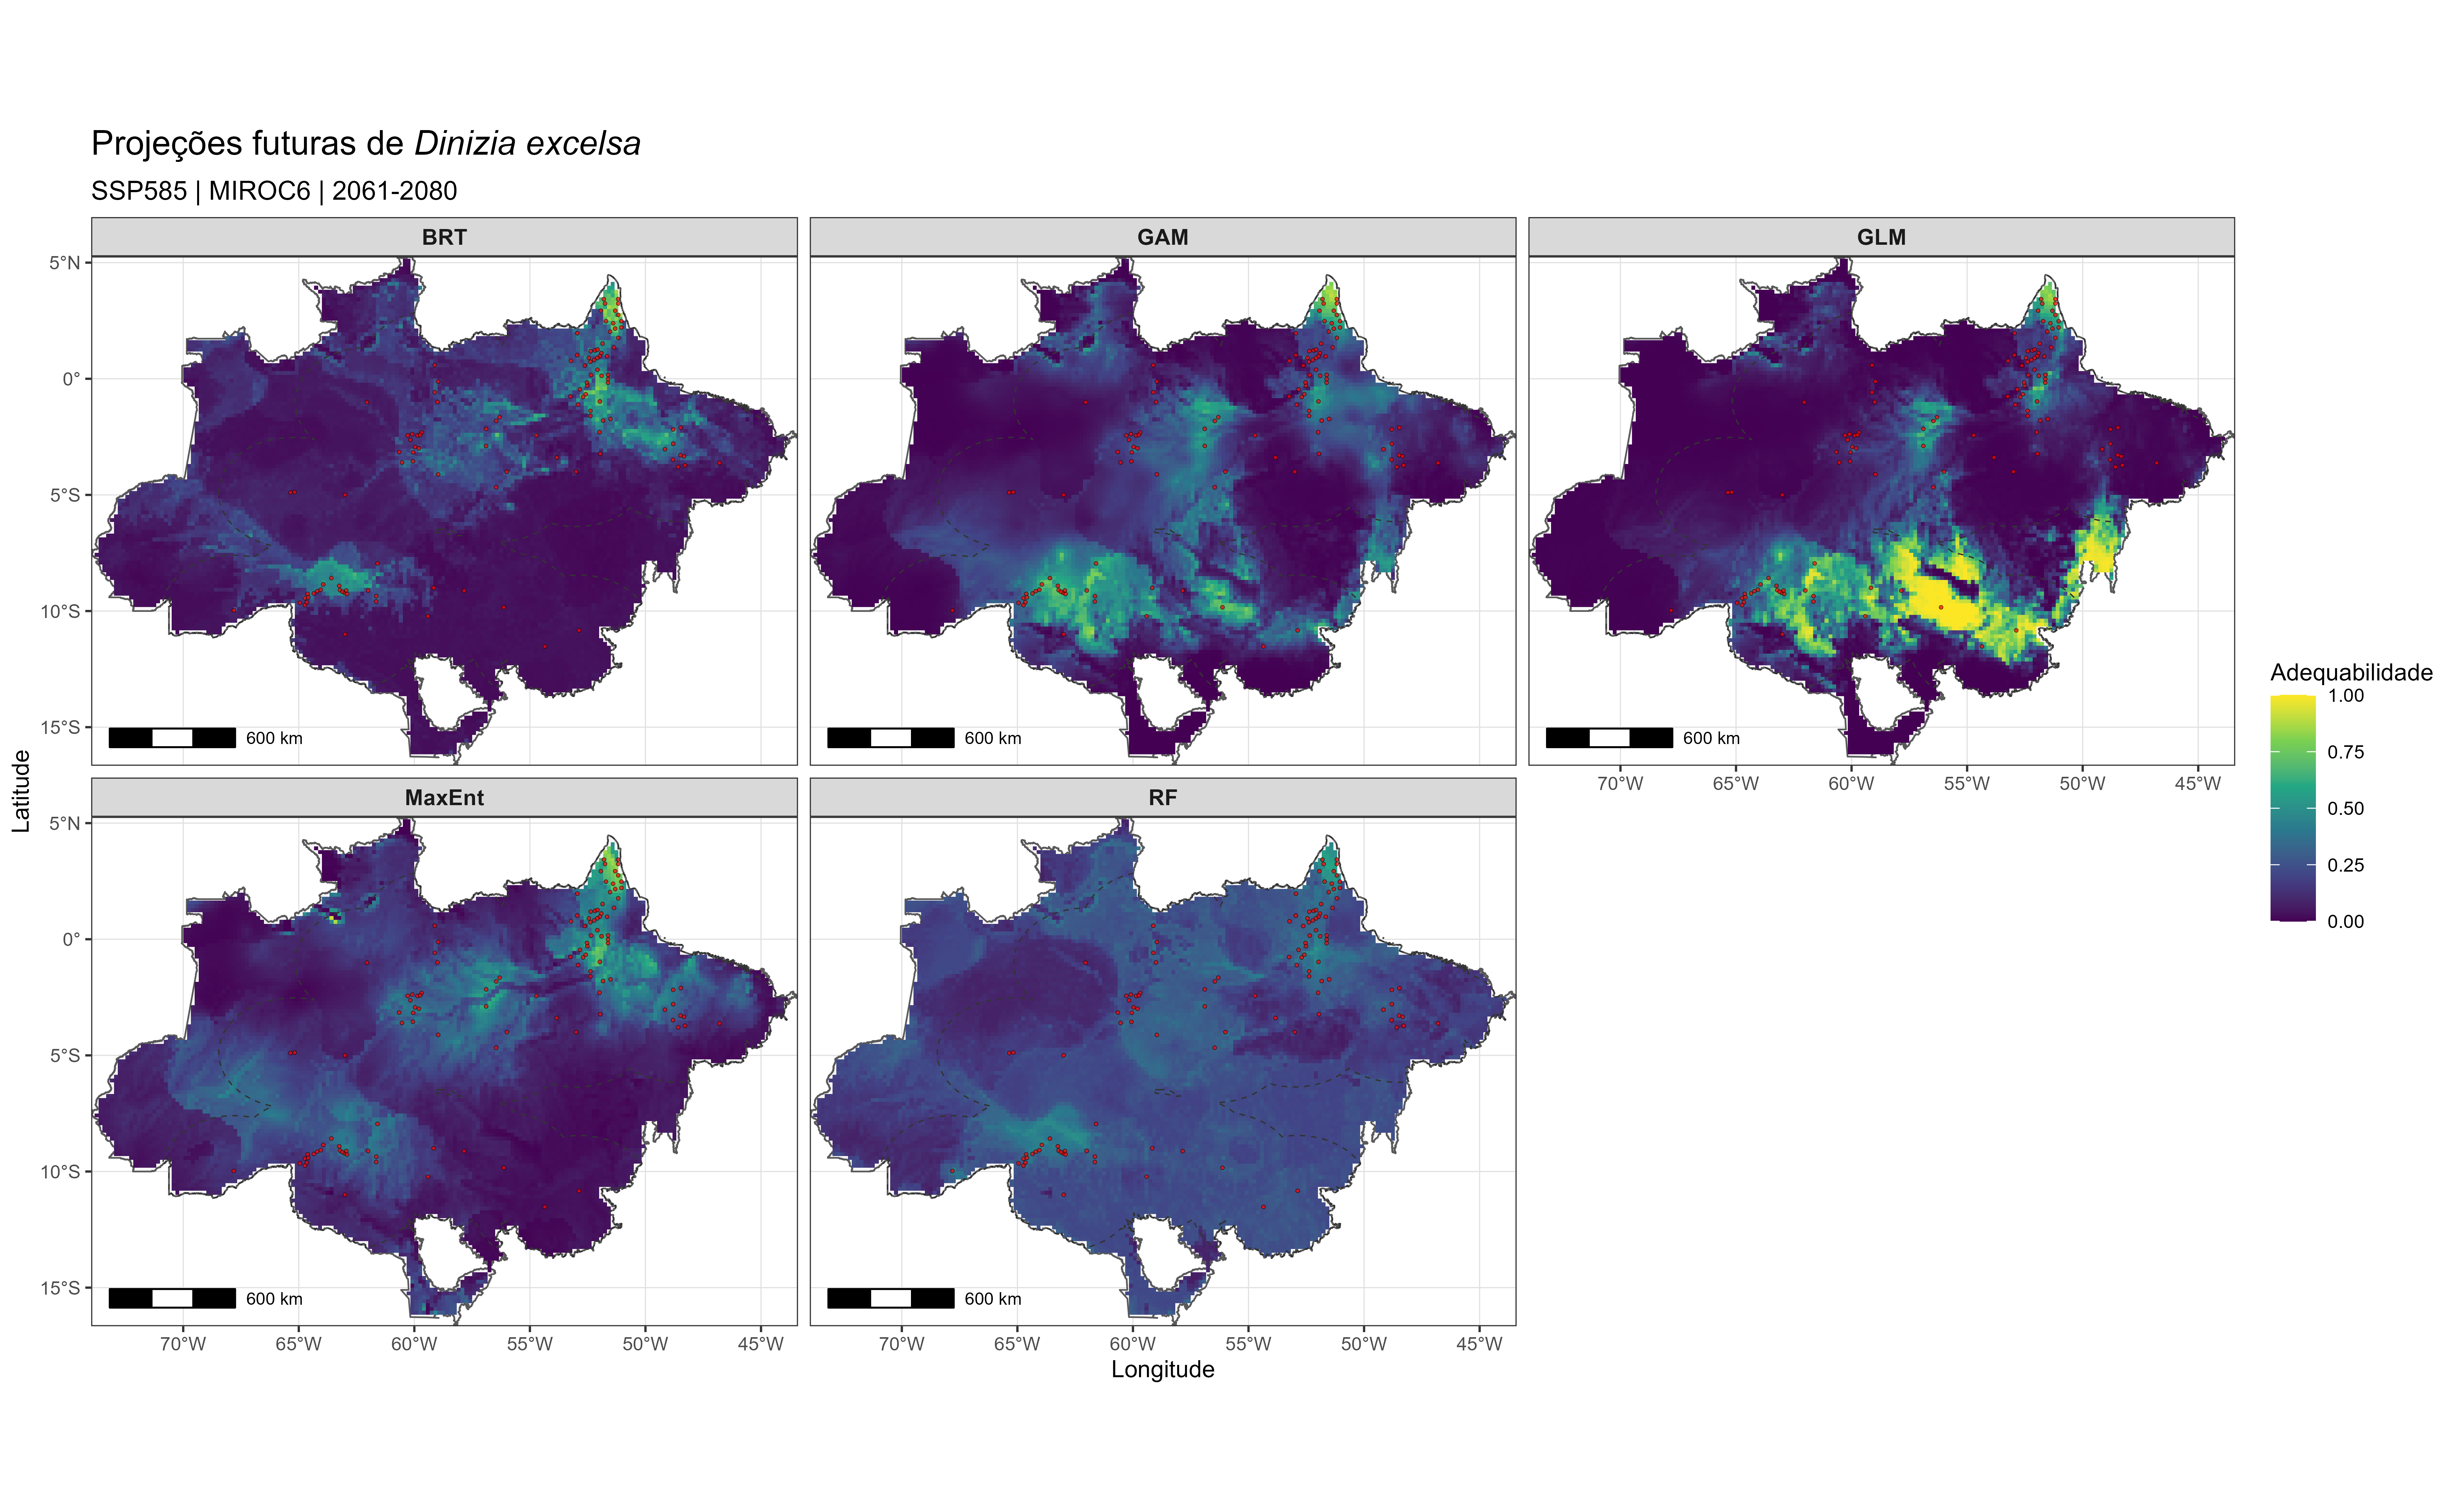
\includegraphics[width=0.98\textwidth]{figuras/unidade13/unidade13_modelos_futuros_ssp585.png}
\caption{Future projections from the individual models for \textit{Dinizia excelsa} under SSP5--8.5. Differences among panels represent algorithmic uncertainty conditional on the same climate scenario.}
\label{fig:unidade13_modelos_futuros}
\end{figure}

\section{Future ensemble projections}

Individual projections are combined into an ensemble for each scenario. An ensemble reduces reliance on a single algorithm and summarizes central tendencies across models, but it does not remove shared biases in occurrences, predictors, sampling, calibration extent, or climate inputs. Model weights and inclusion rules must therefore be fixed transparently and applied consistently across baseline and future conditions.

\rscriptfile{scripts/unidade13/04_ensemble_futuro.R}

\begin{figure}[H]
\centering
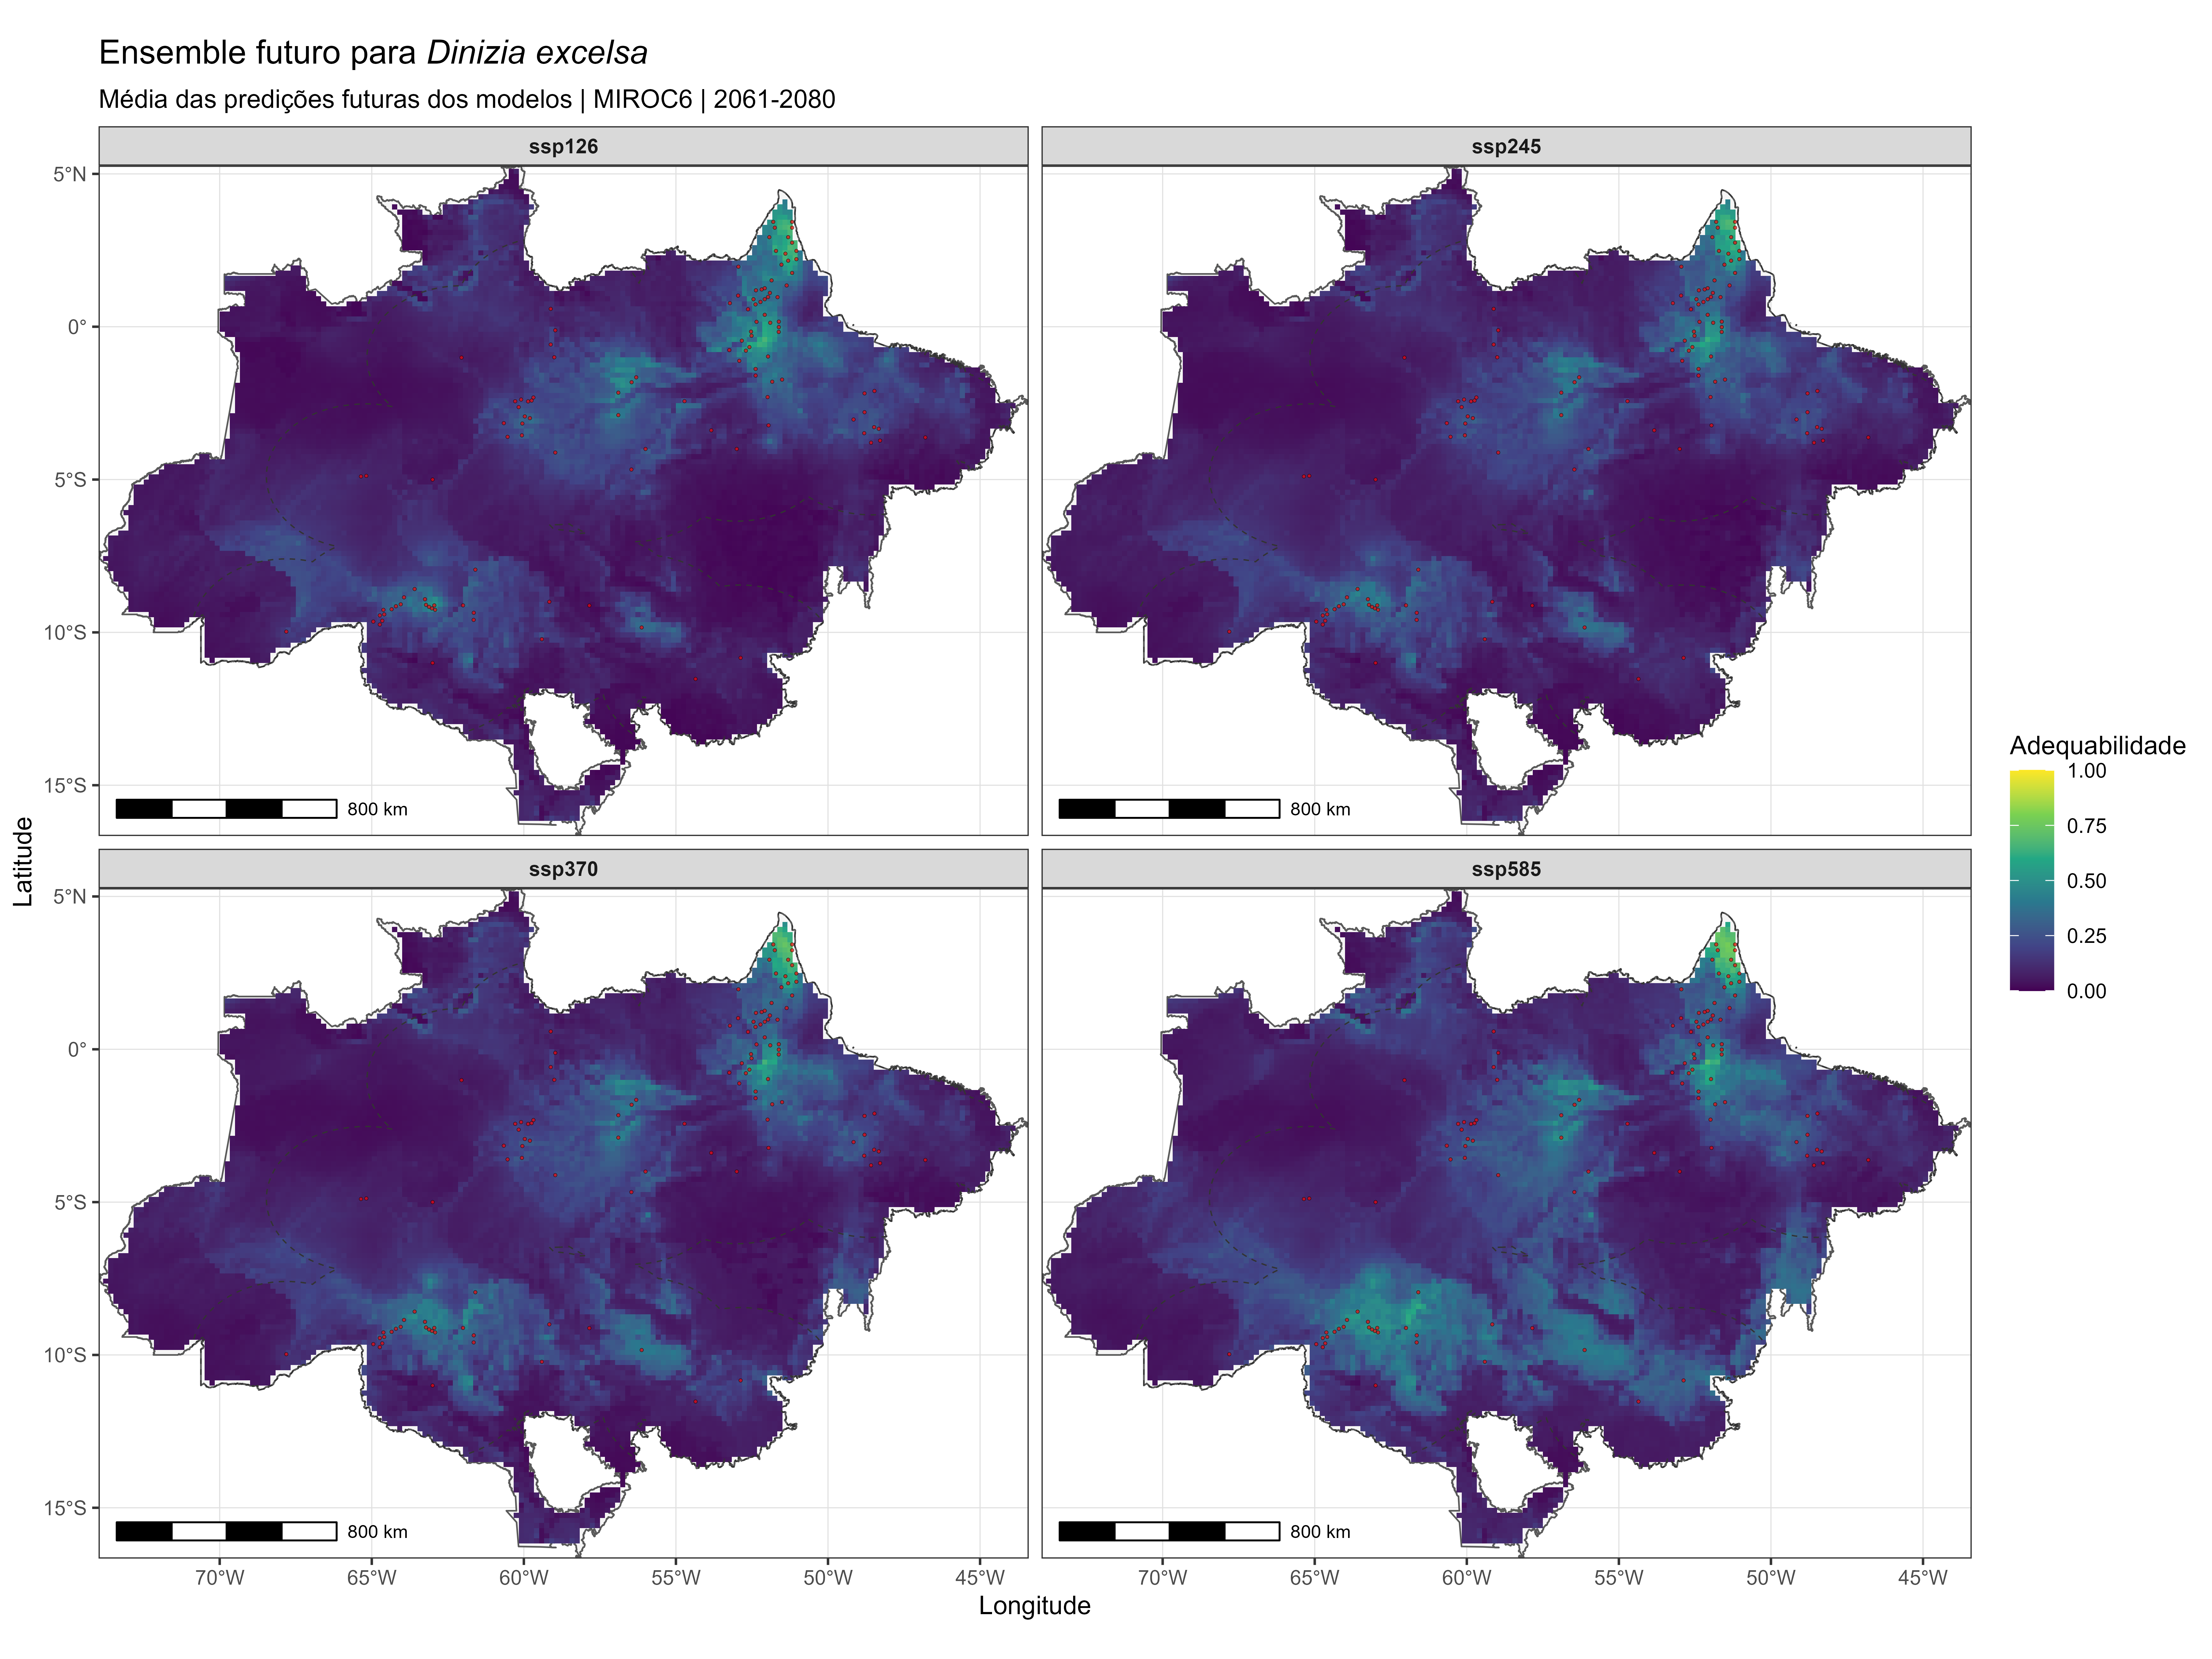
\includegraphics[width=0.96\textwidth]{figuras/unidade13/unidade13_ensemble_futuro_cenarios.png}
\caption{Ensemble projections of future environmental suitability for \textit{Dinizia excelsa} under alternative SSPs.}
\label{fig:unidade13_ensemble_futuro}
\end{figure}

\section{Change in suitability}

Suitability change is calculated as the cellwise difference between future and baseline predictions:

\begin{equationbox}
\[
\Delta S = S_{\mathrm{future}} - S_{\mathrm{baseline}}.
\]
\end{equationbox}

Here, \(S_{\mathrm{future}}\) is the projected suitability for a specified GCM, pathway, and period, and \(S_{\mathrm{baseline}}\) is the estimate for the baseline period. Positive values indicate a relative increase and negative values a relative decrease on the model's output scale. Differences are comparable only when baseline and future predictions were produced with the same fitted model, transformation, and scaling.

\rscriptfile{scripts/unidade13/05_mudanca_adequabilidade.R}

\begin{figure}[H]
\centering
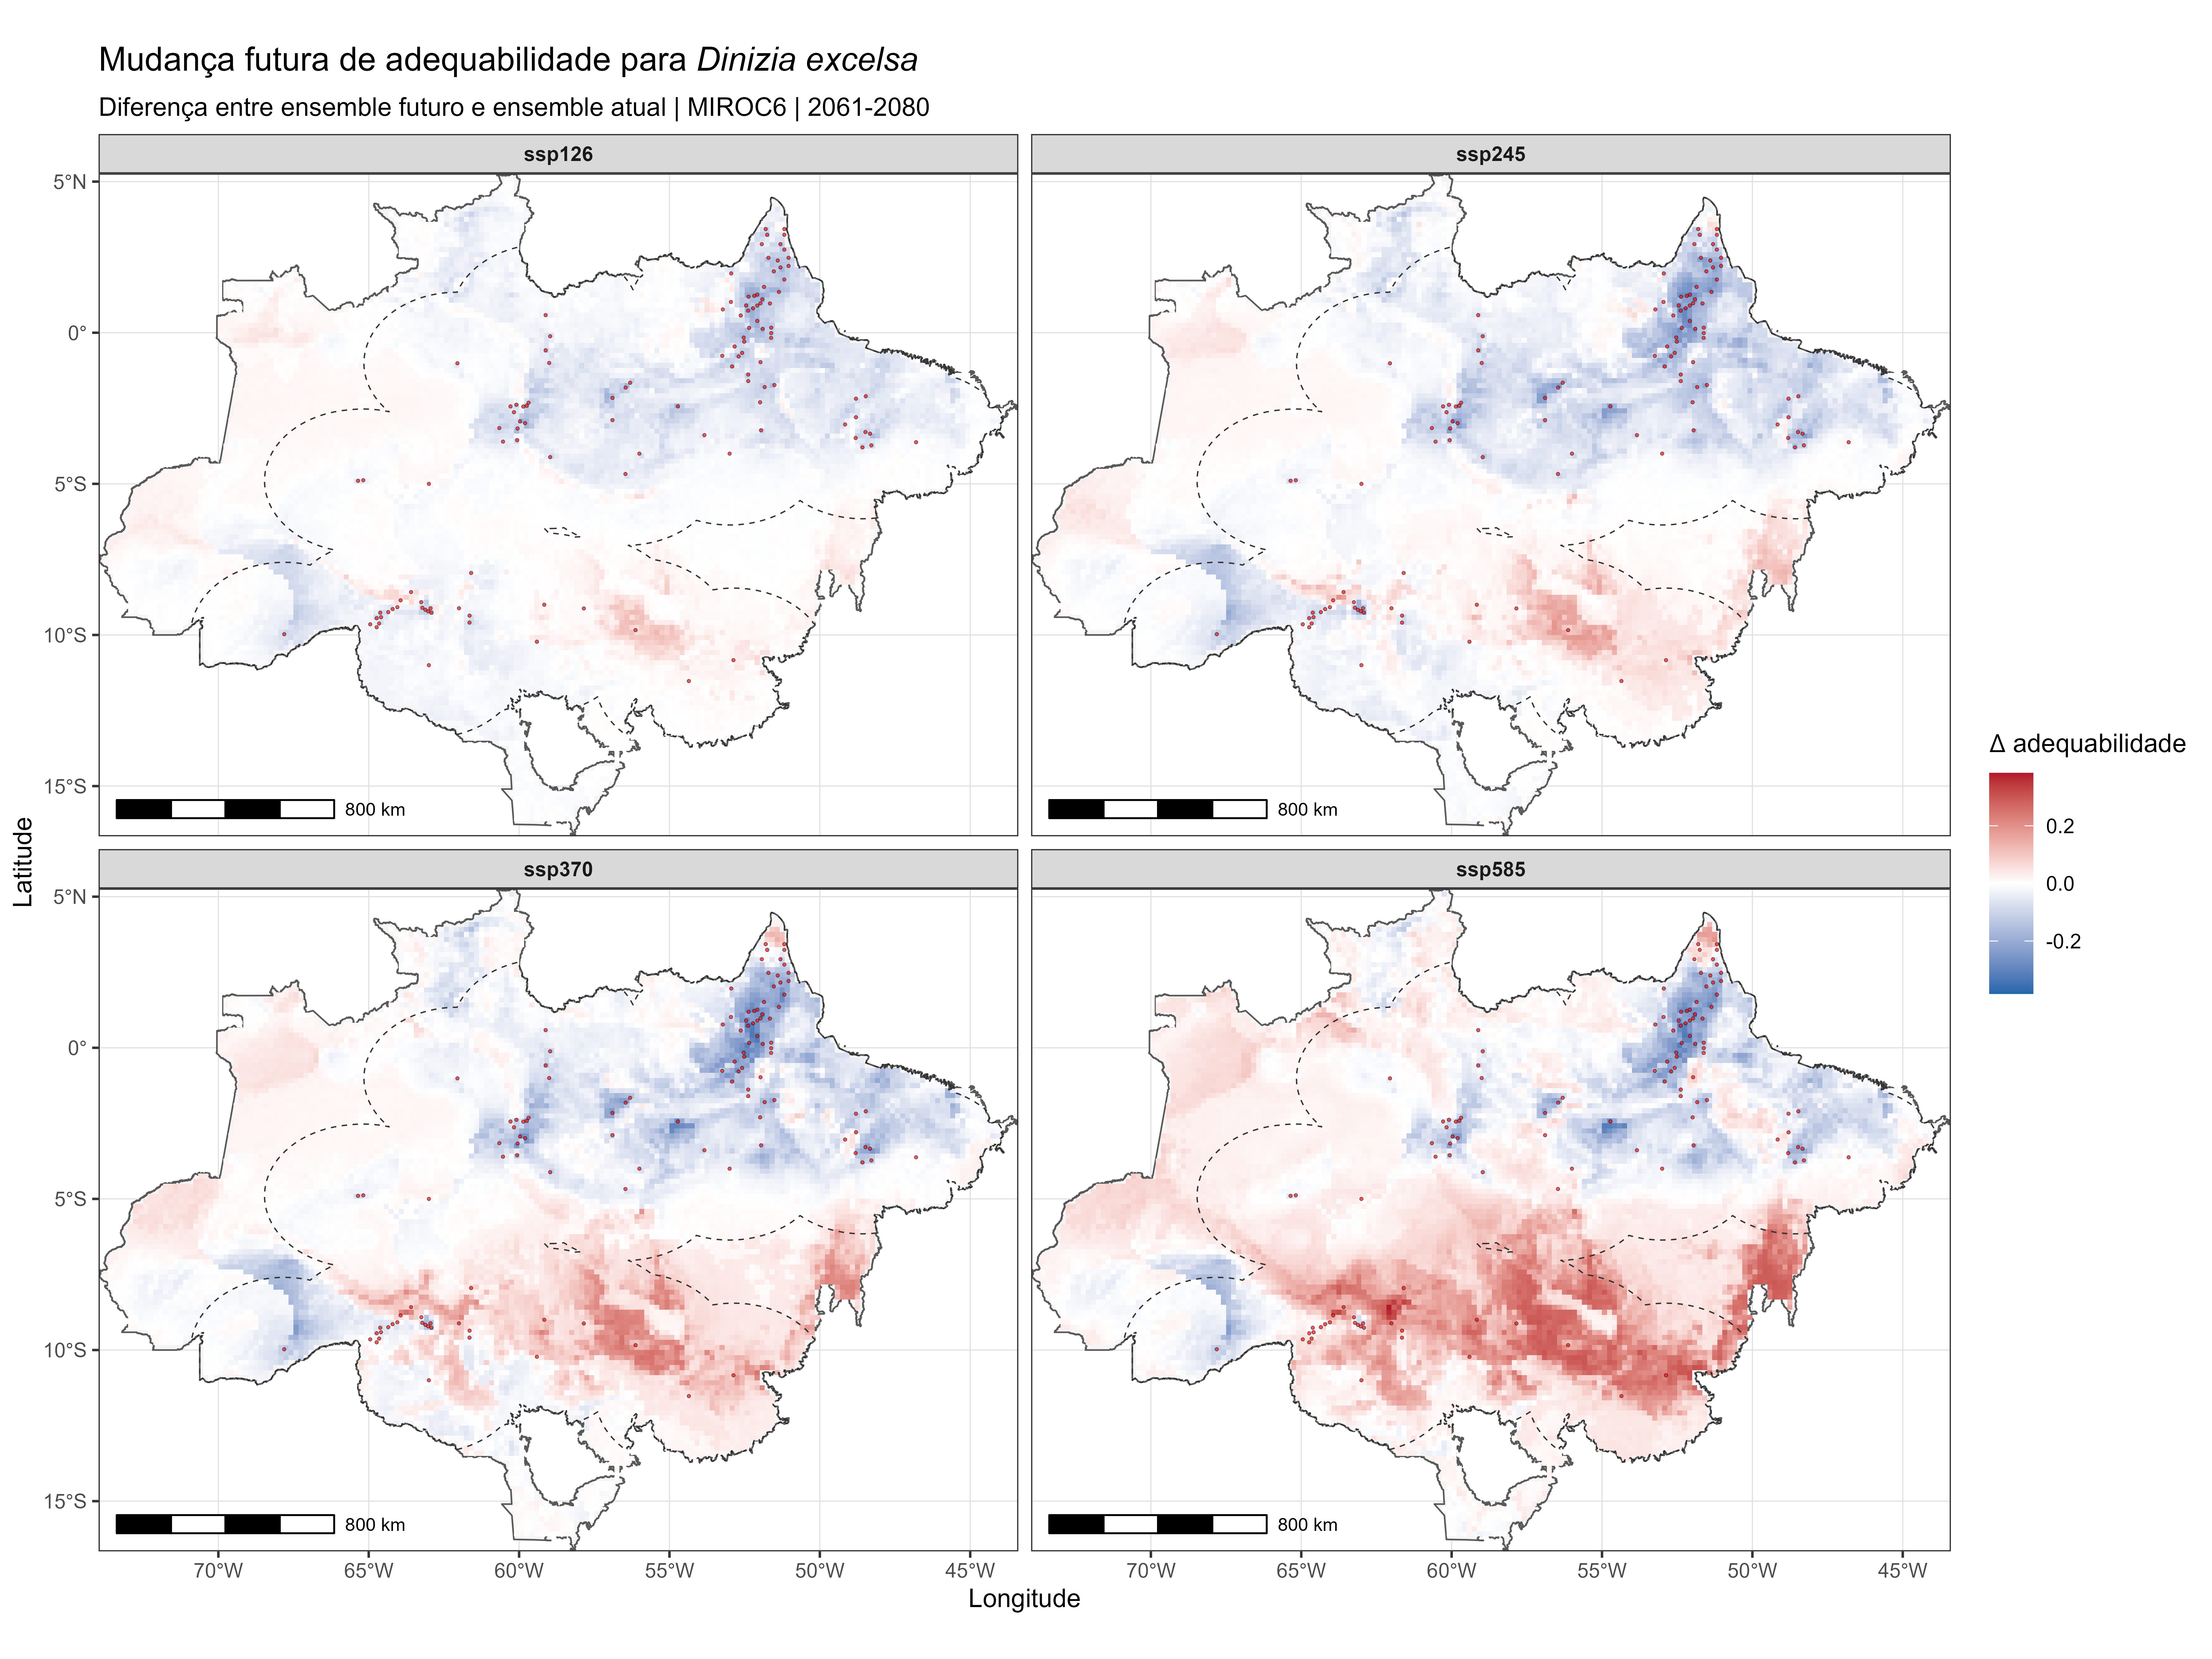
\includegraphics[width=0.96\textwidth]{figuras/unidade13/unidade13_mudanca_adequabilidade.png}
\caption{Projected change in environmental suitability relative to baseline conditions for \textit{Dinizia excelsa}.}
\label{fig:unidade13_mudanca}
\end{figure}

\section{Potential stability, loss, and gain}

Comparing thresholded baseline and future maps classifies cells as stable suitable, potential loss, potential gain, or persistently unsuitable. Because these categories depend on the selected threshold, their areal estimates should be accompanied by the threshold rule and, where feasible, a sensitivity analysis. A potential gain is not equivalent to colonization: accessibility, dispersal, establishment, habitat condition, and biotic constraints must also be considered.

\rscriptfile{scripts/unidade13/06_estabilidade_perda_ganho.R}

\begin{figure}[H]
\centering
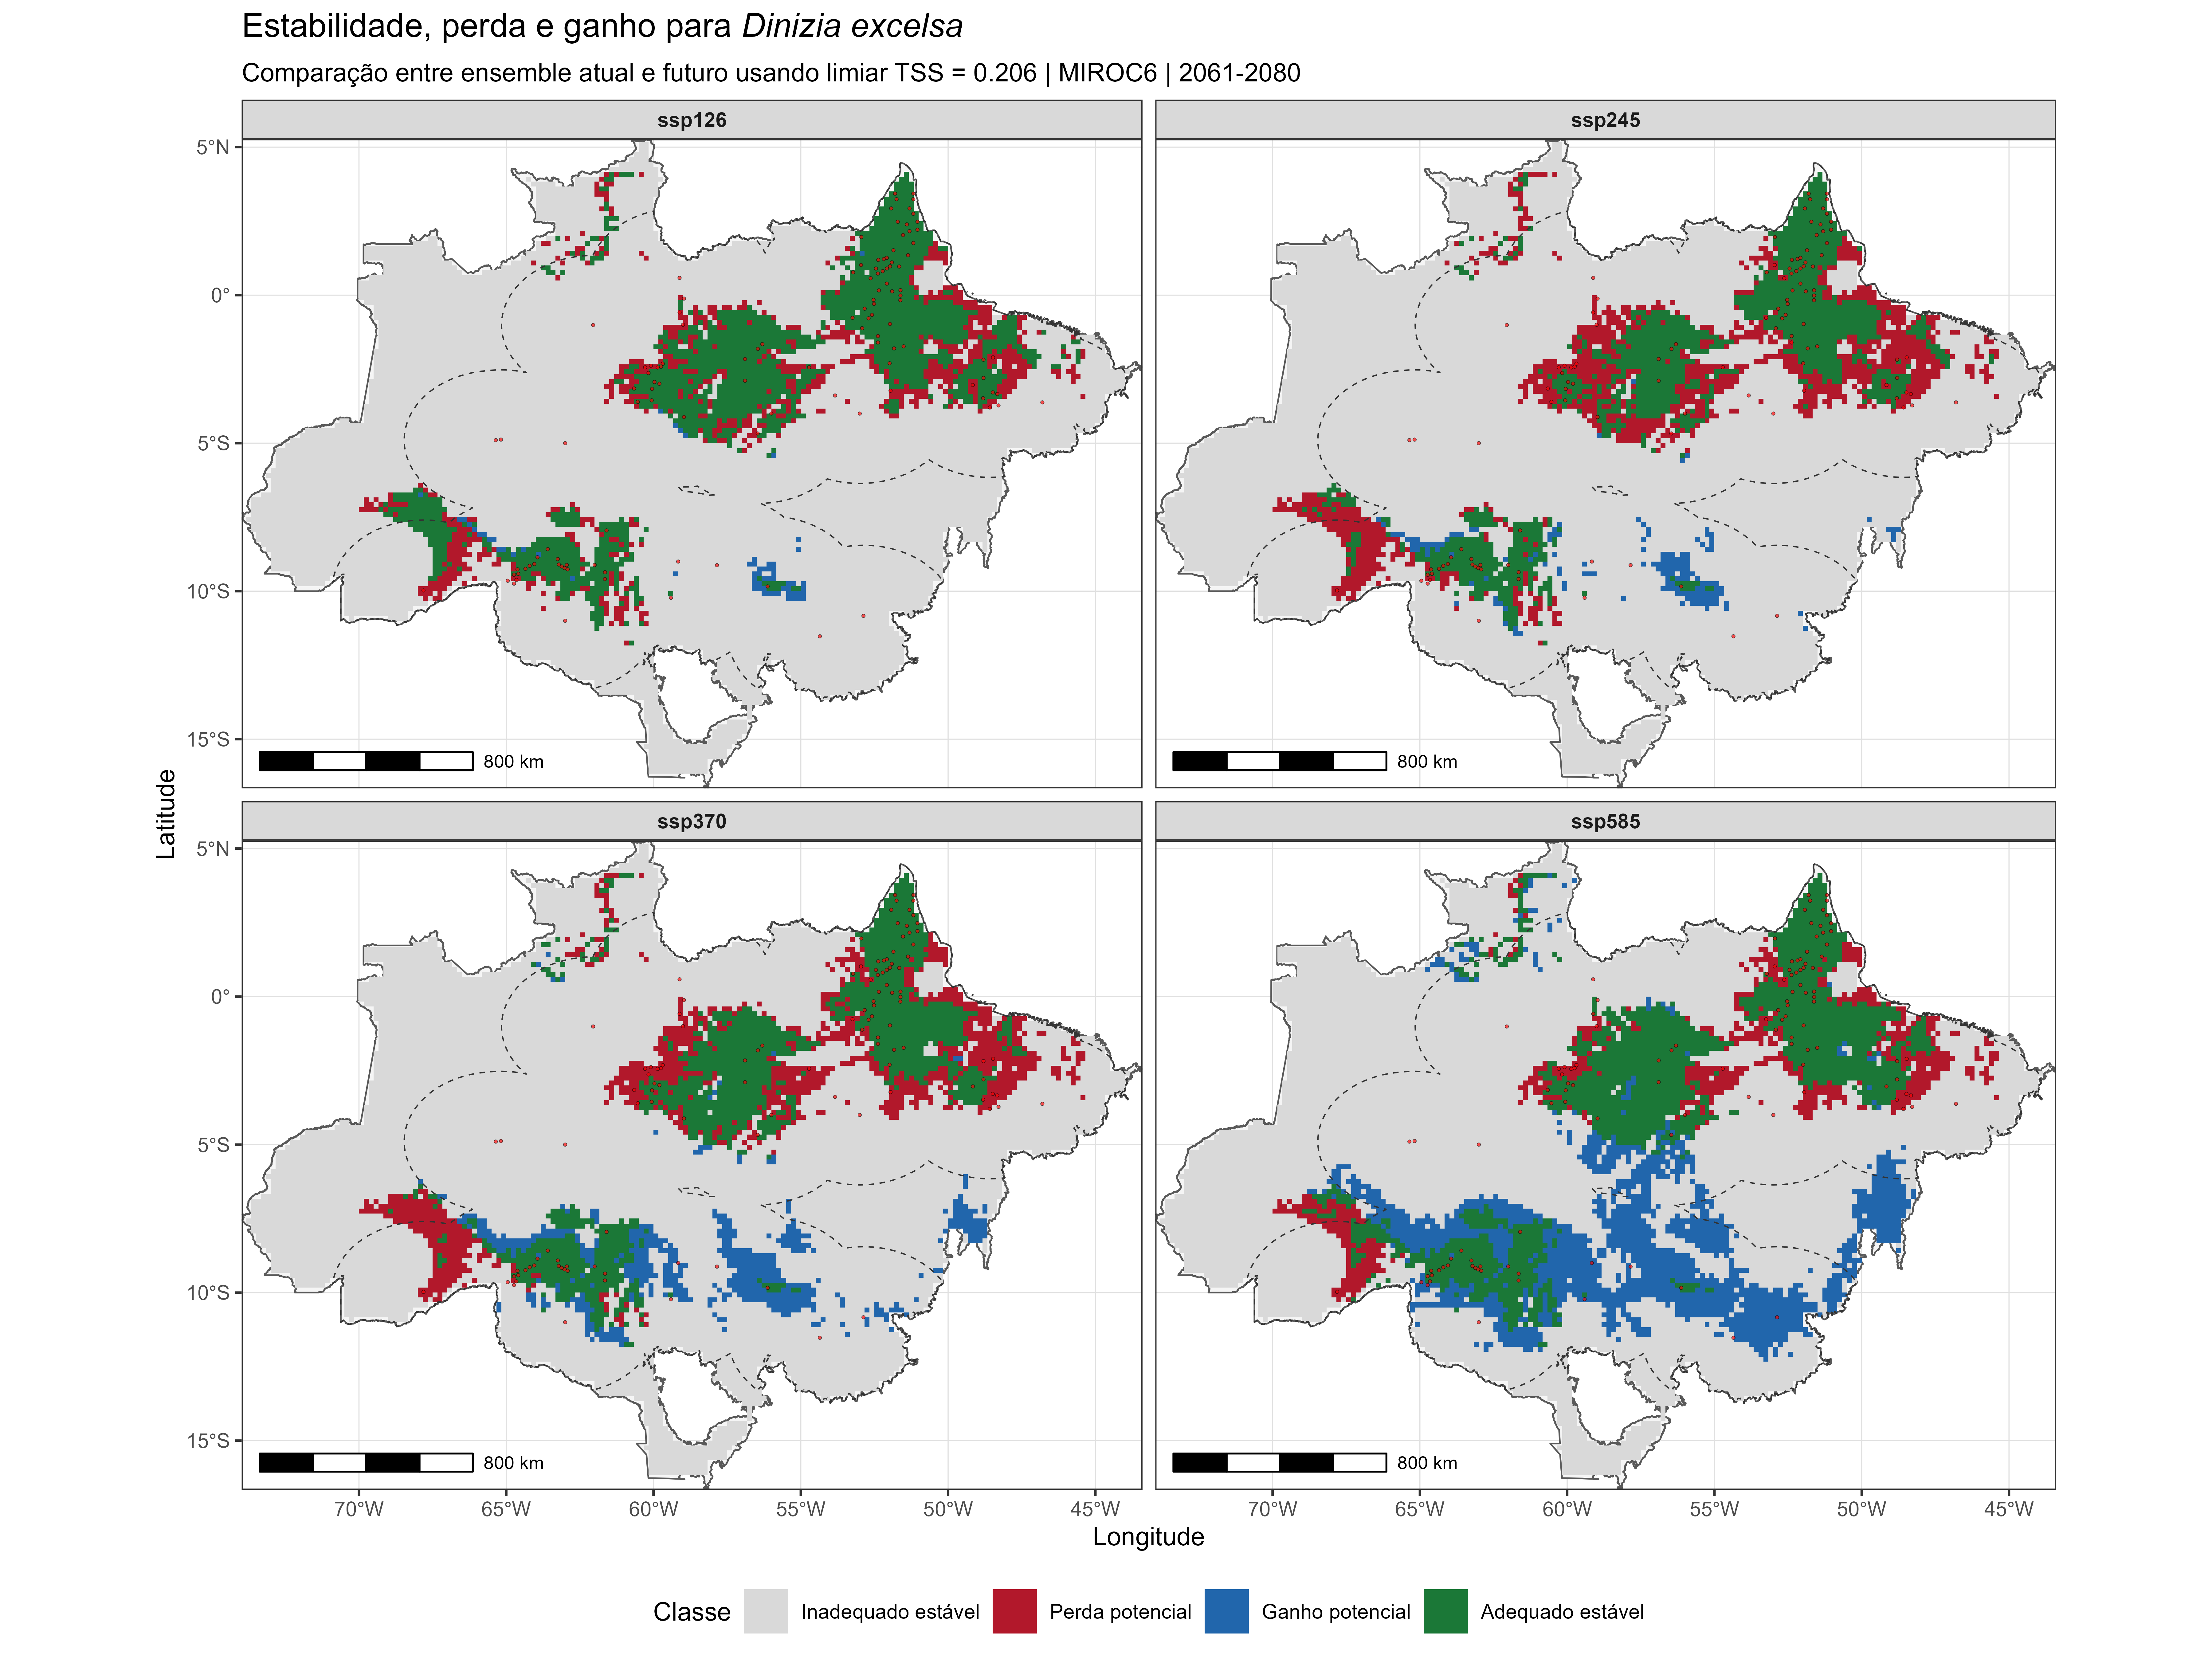
\includegraphics[width=0.96\textwidth]{figuras/unidade13/unidade13_estabilidade_perda_ganho.png}
\caption{Areas of potential stability, loss, and gain in environmental suitability for \textit{Dinizia excelsa} under future scenarios.}
\label{fig:unidade13_estabilidade}
\end{figure}

\section{Tabular synthesis across scenarios}

\rscriptfile{scripts/unidade13/07_sintese_cenarios_futuros.R}

\begin{figure}[H]
\centering
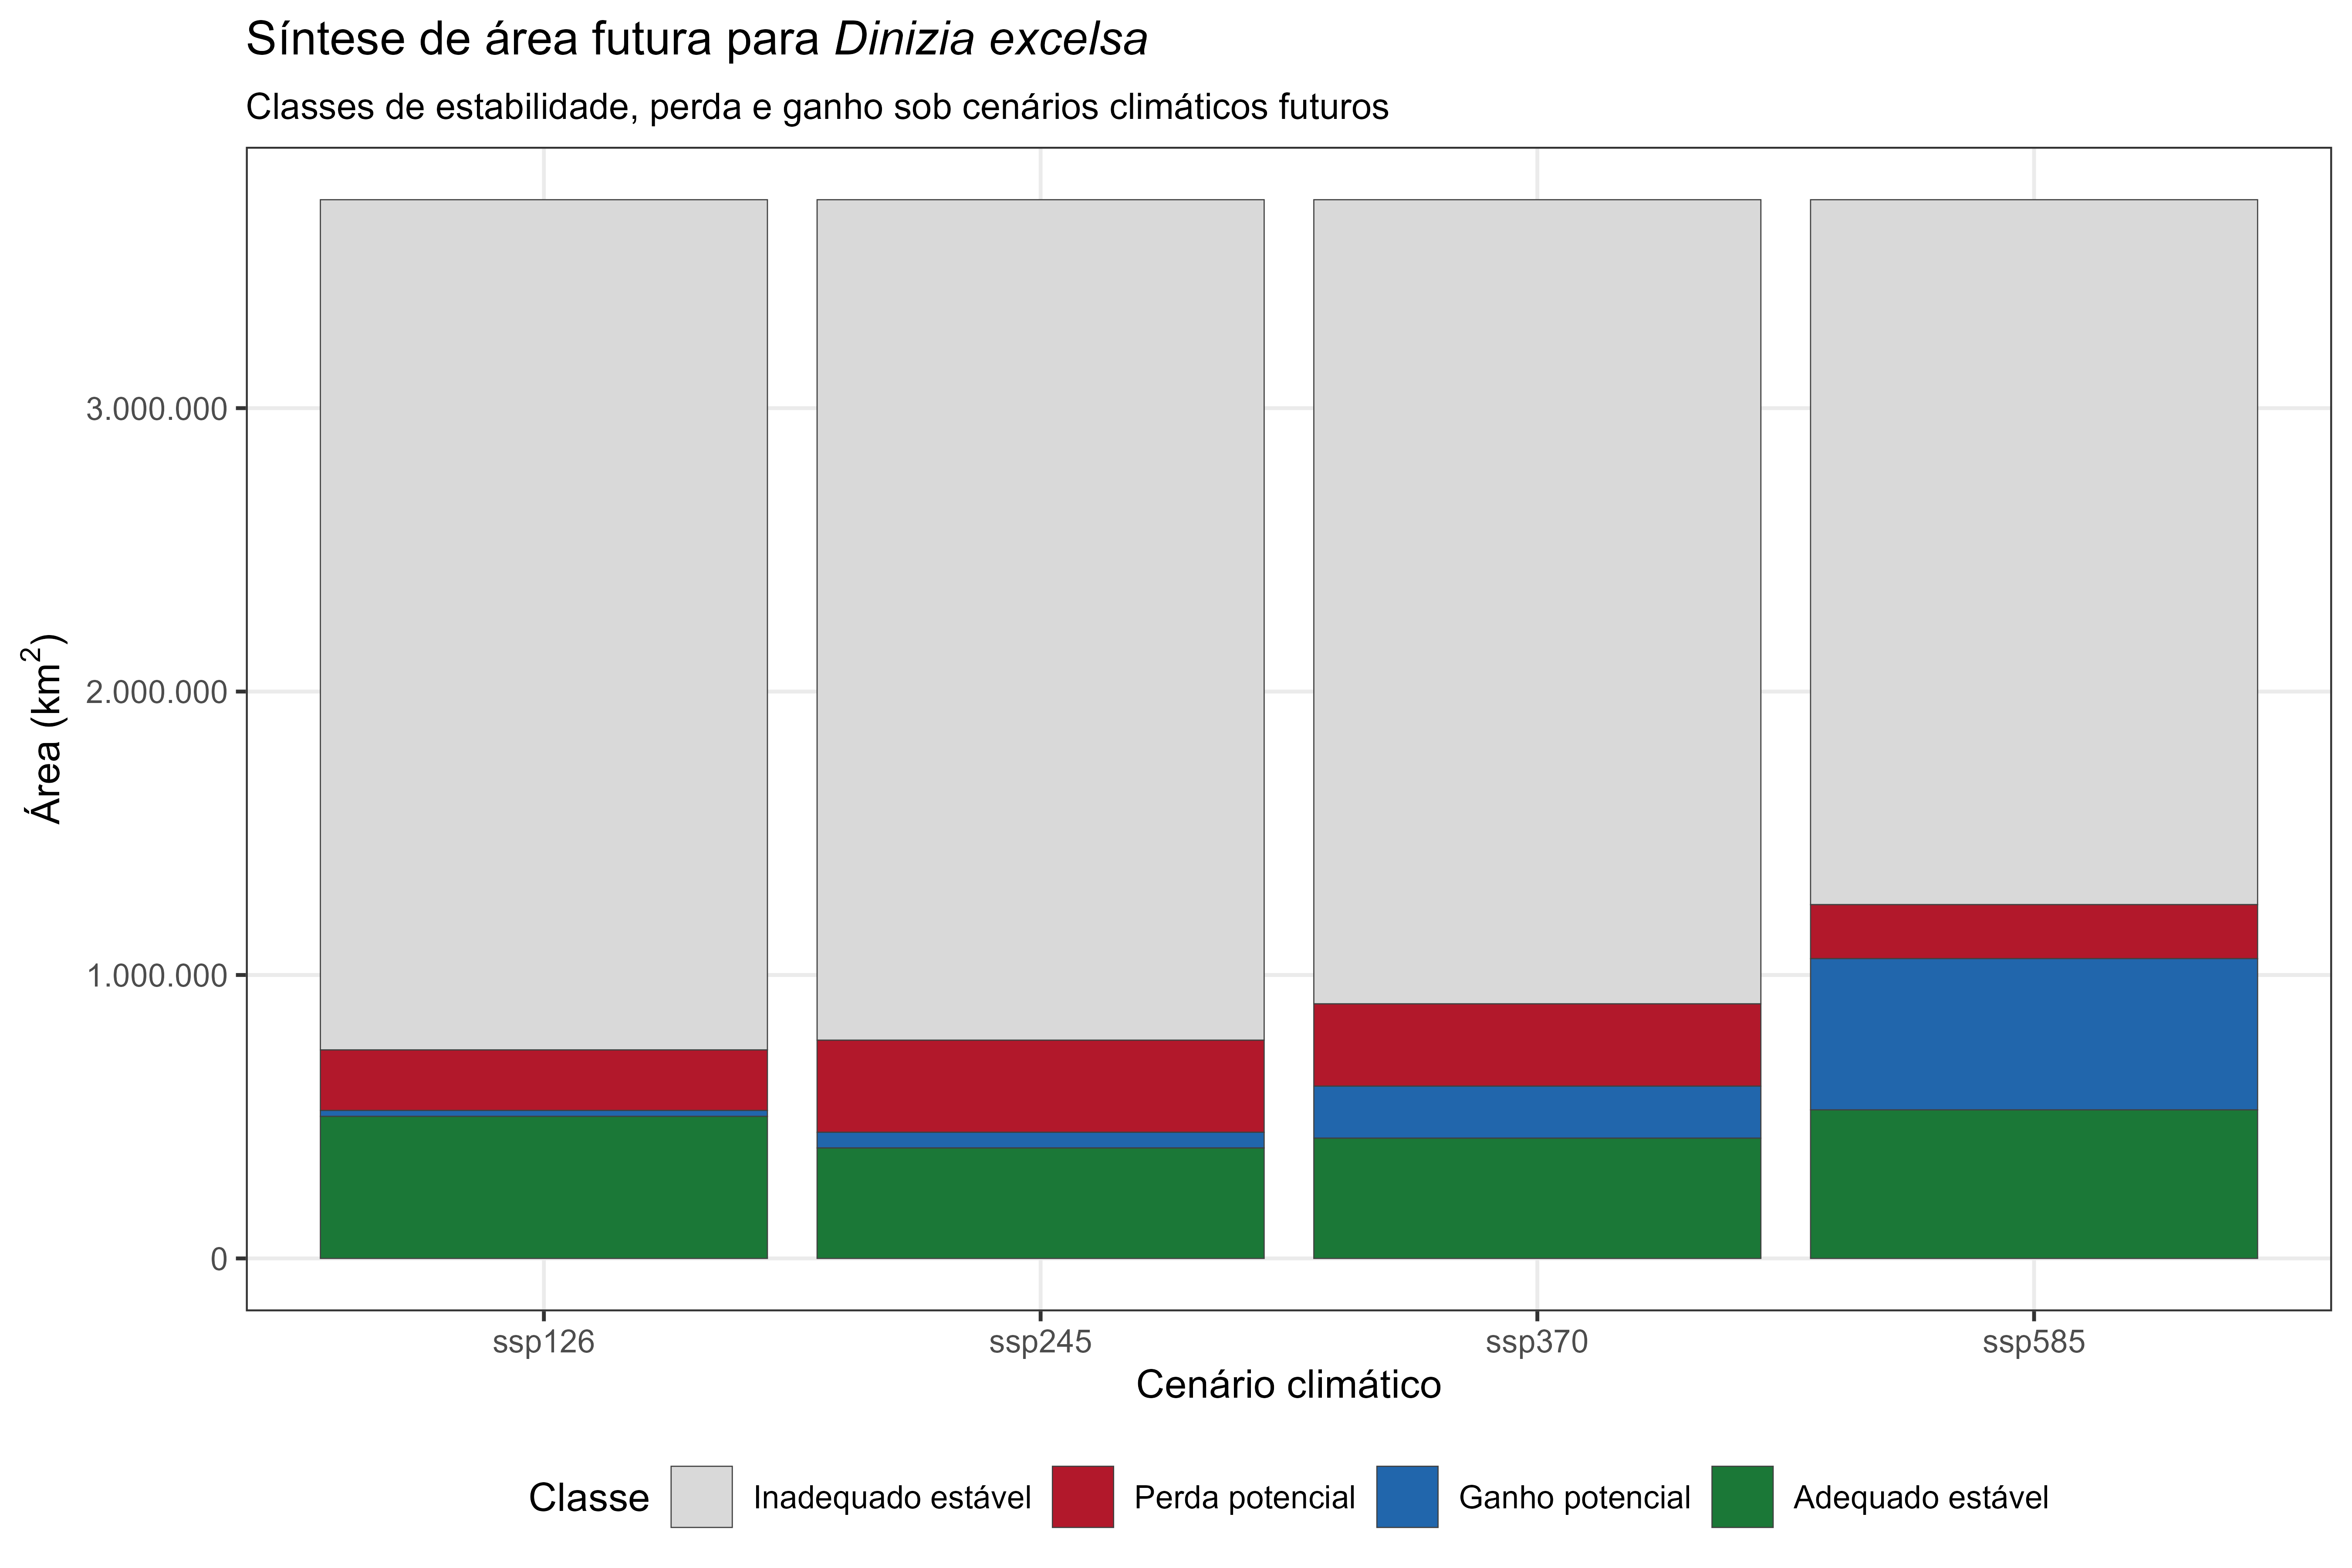
\includegraphics[width=0.88\textwidth]{figuras/unidade13/unidade13_sintese_area_adequada.png}
\caption{Estimated baseline and future suitable area for \textit{Dinizia excelsa} under alternative SSPs.}
\label{fig:unidade13_sintese_area}
\end{figure}

Area summaries should retain the full hierarchy of uncertainty wherever the data permit: algorithm, GCM, SSP, time horizon, replicate or fold, and threshold. Reporting only an ensemble mean can conceal disagreement that is directly relevant to conservation decisions.

\section{Complete pipeline}

\rscriptfile{scripts/unidade13/08_pipeline_projecoes_futuras.R}

\section{Chapter synthesis}

Future climate projections provide conditional evidence about possible changes in environmental suitability under alternative climate trajectories. For \textit{Dinizia excelsa}, they support questions about climatic persistence, potential contraction or expansion, environmental stability, and exposure to warming. They do not, by themselves, predict future occupancy or population viability.

\begin{conceito}[title={\faBook\quad Key message}]
Future SDM outputs are scenarios of environmental suitability, not deterministic forecasts of occurrence. Defensible inference depends on baseline data quality, predictor comparability, explicit scenario design, transferability diagnostics, and propagation of uncertainty across algorithms and climate models.
\end{conceito}

\section{Review exercises}

\begin{enumerate}
\item Distinguish baseline climate data from future climate projections in an SDM workflow.
\item What information is encoded in an SSP-based scenario label such as SSP2--4.5?
\item Why must future predictors match the variables used for model calibration in definition and units, not merely in name?
\item How should positive and negative values of \(\Delta S\) be interpreted?
\item What does climatic stability mean in a comparison of thresholded maps?
\item Why should potential gains not be interpreted as certain future colonization?
\item How can an uncertainty hierarchy improve the conservation use of future projections?
\end{enumerate}
